\documentclass[12pt,a4paper]{report}
\usepackage[utf8]{inputenc}
\usepackage{amsfonts}
\usepackage{amssymb}
\usepackage{graphicx}
\usepackage{float}

% sets margin
\usepackage[hmargin=3cm,vmargin=2.5cm]{geometry}

% creates landscape pages
\usepackage{pdflscape}
\usepackage{pdfpages}

% defining settings for textpos
\usepackage[absolute]{textpos}
\setlength{\TPHorizModule}{\paperwidth}
\setlength{\TPVertModule}{\paperheight}

% headers / footers
\usepackage{fancyhdr}
\pagestyle{fancy}
\fancyhf{}
\rhead{Assignment 1a}
\lhead{CSG1132: Communicating in an IT Environment}
\rfoot{\thepage}
\lfoot{Martin Ponce, ID: 10371381}
\renewcommand{\footrulewidth}{0.5pt}

% defining landscape headers / footers
\fancypagestyle{fancylscape}{
	\fancyhf{}
	\renewcommand{\footrulewidth}{0pt}
	\renewcommand{\headrulewidth}{0pt}
	% header
	\begin{textblock}{0.05}[-0.5,-2](0,0)
		{\rotatebox{90}{CSG1132: Communicating in an IT Environment}}
	\end{textblock}
		\begin{textblock}{0.05}[-0.5,-1](0,0)
		{\rotatebox{90}{Assignment 1a}}
	\end{textblock}
	\begin{textblock}{0.05}[-1,-0.109](0,0)
		{\rotatebox{90}{\rule{24.2cm}{0.5pt}}}
	\end{textblock}
	% footer
	\begin{textblock}{0.05}[-19,-4.28](0,0)
		{\rotatebox{90}{Martin Ponce, ID: 10371381}}
	\end{textblock}
		\begin{textblock}{0.05}[-19,-12.8](0,0)
		{\rotatebox{90}{\thepage}}
	\end{textblock}
		\begin{textblock}{0.05}[-18.7,-0.109](0,0)
		{\rotatebox{90}{\rule{24.2cm}{0.5pt}}}
	\end{textblock}
}

% adjusts padding between caption and figure
\setlength{\belowcaptionskip}{5pt}

% adds links to references and colors them blue
\usepackage{hyperref}
\hypersetup{colorlinks=true,
			linkcolor=blue,
			citecolor=blue,
			urlcolor=blue}

% apa style referencing
\usepackage[sectionbib, natbibapa]{apacite}
\usepackage{chbibref}

% front matter
\title{Edith Cowan University\\CSG1132\\Communicating in an IT Environment\\Assignment 1a}
\author{Concept Map, Thesis Statements \& Learner Reflection\\\\
		Martin Ponce\\Student 10371381\\\\Tutor: Dr. Mark Brogan}
\date{August 24, 2014}

\begin{document}

% title page
\maketitle

% toc
\tableofcontents
\thispagestyle{fancy}

\newpage
\section*{\textsf{Task 1: Concept Map}}
\addcontentsline{toc}{section}{Task 1: Concept Map}

\subsection*{\textsf{Focus Question:}}
What is the role of psychology in personal use of Facebook?\\

See \emph{Figure 1.}

\subsection*{\textsf{Concept Map Reference List}}
\begin{itemize}
\item \citet*{Pai2013}
\item \citet*{McAndrew2012}
\item \citet*{Nadkarni2012}
\item \citet*{Moore2012}
\item \citet*{Ross2009}
\item \citet*{Toma2013}
\item \citet*{Ellison2007}
\item \citet*{Park2011}
\item \citet*{Anderson2012}
\item \citet*{Ku2013}
\item \citet*{Rosen2013}
\item \citet*{Trottier2012}
\item \citet*{Kwan2013}
\end{itemize}

\newpage
\begin{landscape}
	\begin{figure} % empty figure, just using to add caption
		\centering
		\caption{Concept map}
	\end{figure}
	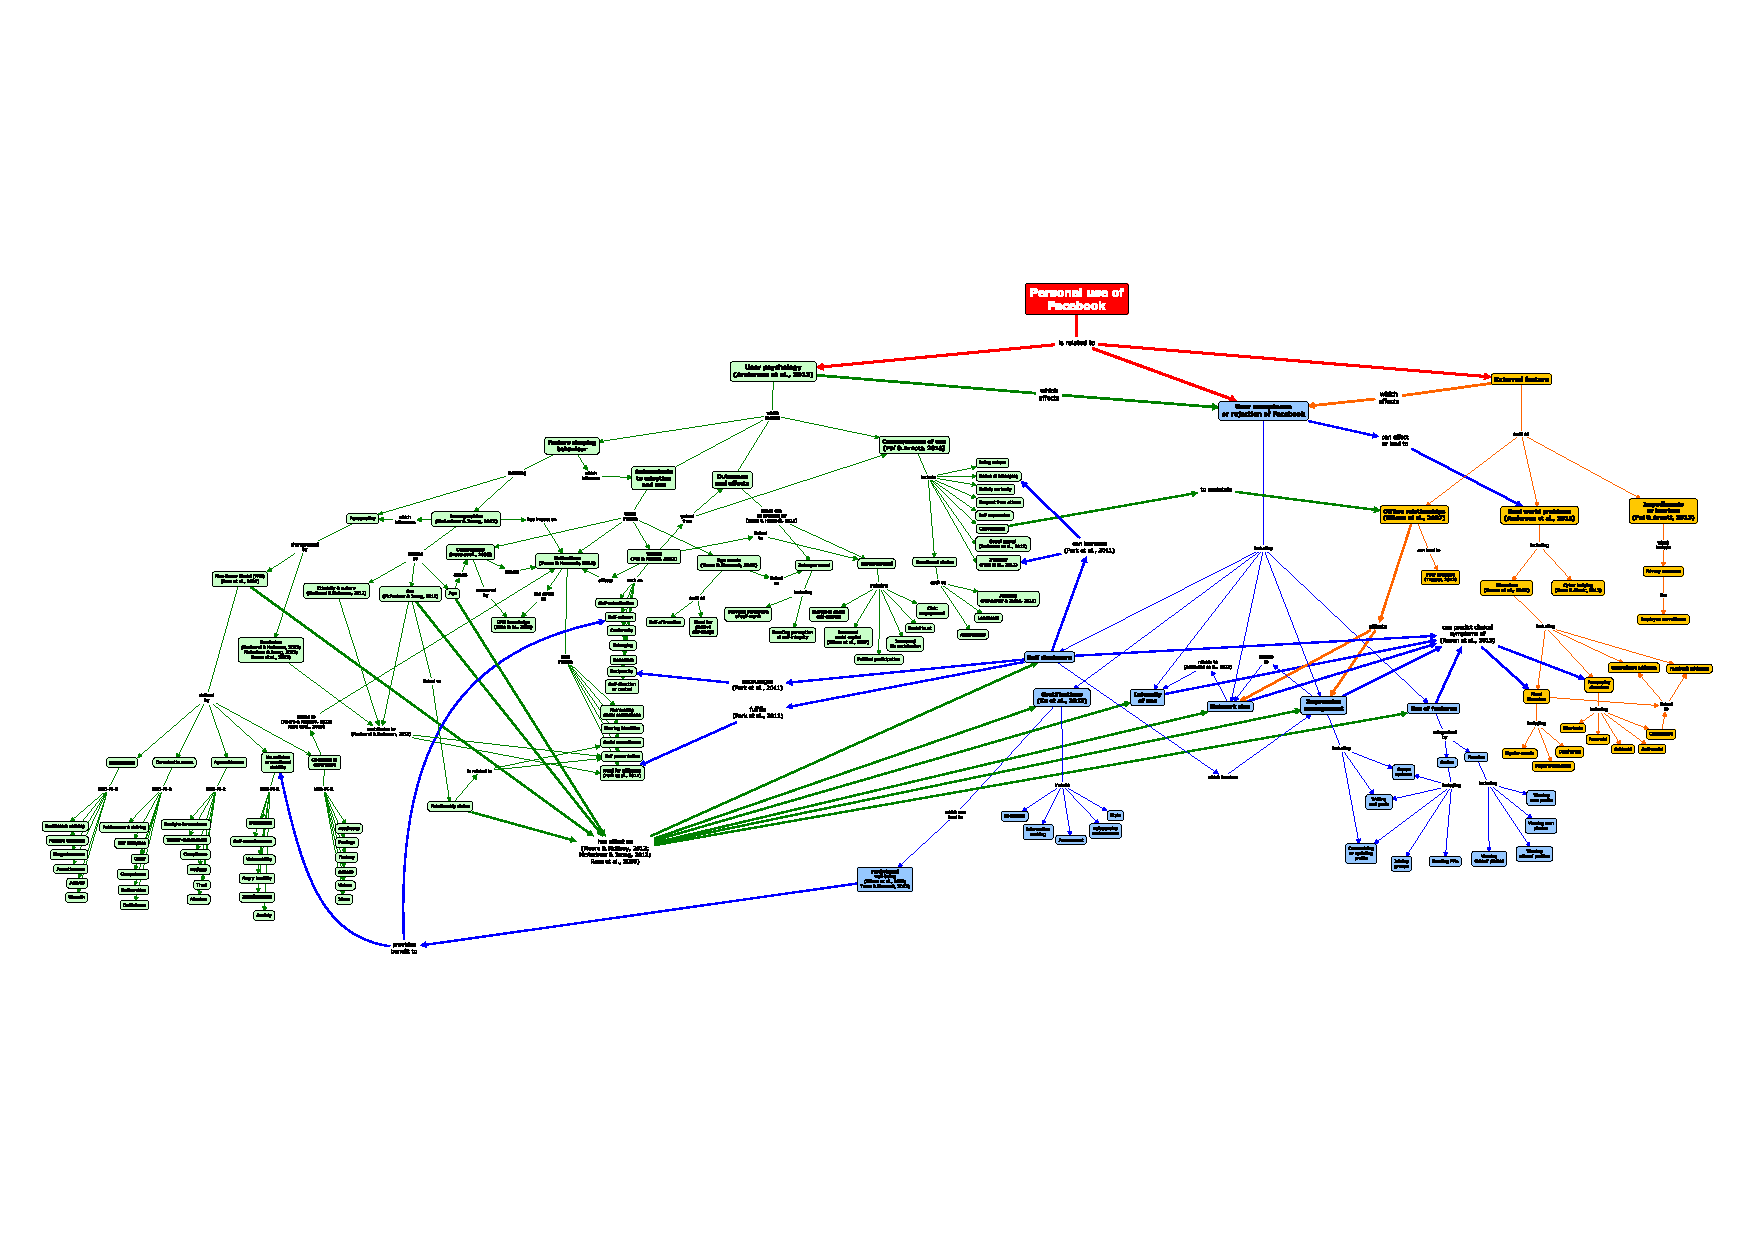
\includepdf[landscape, turn=true, pagecommand={\thispagestyle{fancylscape}}]{./img/CSG1132_Facebook_Cmap_v9.pdf}
\end{landscape}

%\begin{landscape}
%\begin{figure}[H]
%	\centering
%	\caption{Concept map}
%	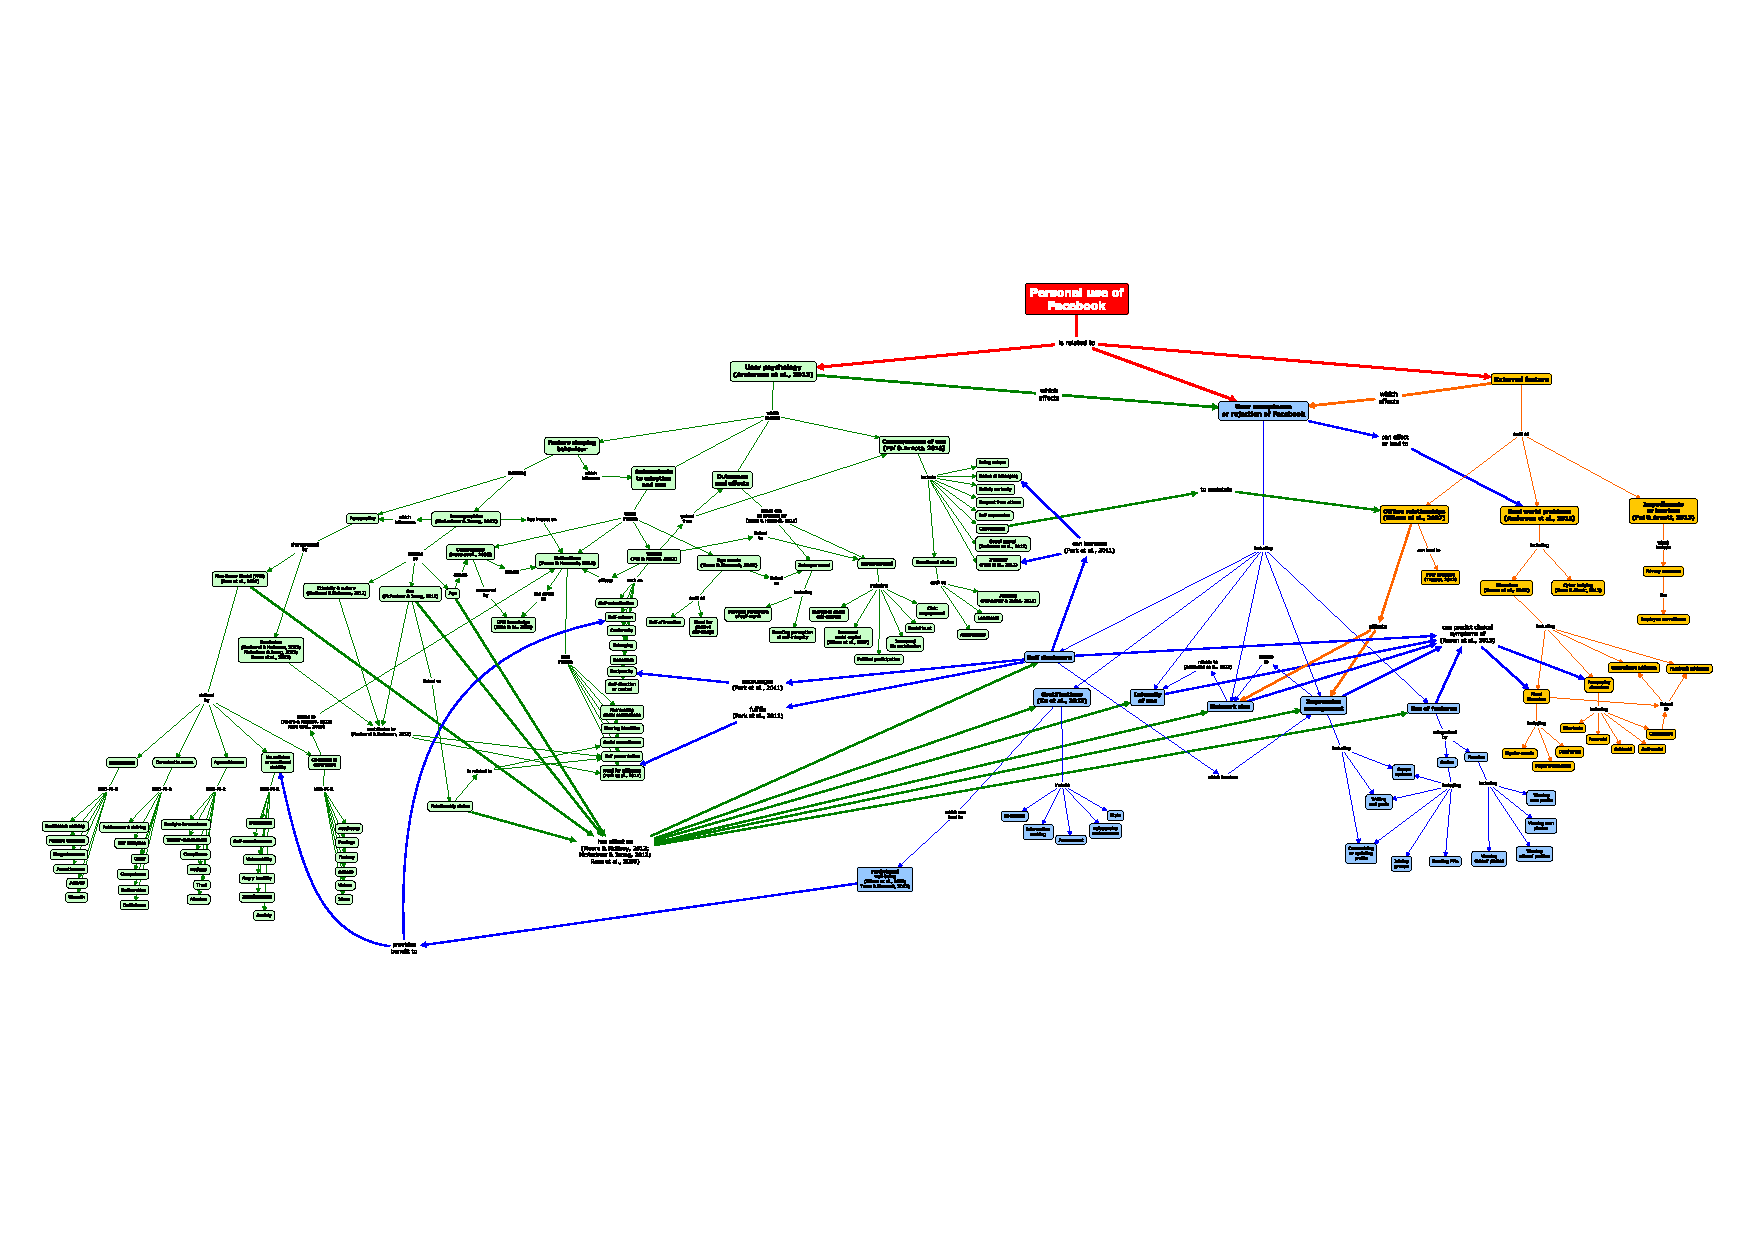
\includepdf[landscape, turn=false]{./img/CSG1132_Facebook_Cmap_v9.pdf}
%	\thispagestyle{fancylscape}
%\end{figure}
%\end{landscape}

\newpage
\section*{\textsf{Task 2: Thesis Statements}}
\addcontentsline{toc}{section}{Task 2: Thesis Statements}

\subsection*{\textsf{Argumentative Statement}}

\subsubsection*{\textsf{Question:}}

Can a user's relationship status affect their usage of Facebook? \citep{McAndrew2012}.

\subsubsection*{\textsf{Statement Draft/s:}}
\begin{enumerate}
\item A user's relationship status as a behaviour modifier on Facebook.
\item The relationship status as a predicator of Facebook use.
\item The relationship status: Modifying user behaviour on Facebook.
\end{enumerate}

\subsubsection*{\textsf{Final Argumentative Statement:}}
User behaviour on Facebook is modified by their relationship status.

\subsection*{\textsf{Analysis Statement}}

\subsubsection*{\textsf{Question:}}
What are the motivations for self-disclosure on Facebook? \citep{Park2011}.

\subsubsection*{\textsf{Statement Draft/s:}}
\begin{enumerate}
\item Self-disclosure on Facebook fulfils the human need for affiliation.
\end{enumerate}

\subsubsection*{\textsf{Final Analysis Statement:}}
Facebook self-disclosure and its relation to the human need for affiliation.

\subsection*{\textsf{Exposition Statement}}

\subsubsection*{\textsf{Question:}}
What are the psychological benefits in the use of Facebook? \citep{Toma2013}.

\subsubsection*{\textsf{Statement Draft/s:}}
\begin{enumerate}
\item The positive psychological effects of Facebook use.
\end{enumerate}

\subsubsection*{\textsf{Final Exposition Statement:}}
The positive psychological effects of Facebook use are increased perceptions of self-worth and self-integrity.

\newpage
\section*{\textsf{Task 3: Summary \& Learner Reflection}}
\addcontentsline{toc}{section}{Task 3: Summary \& Learner Reflection}

\subsection*{\textsf{Concept Map Summary}}
\addcontentsline{toc}{subsection}{Concept Map Summary}

The concept map was developed in 1972 by researchers at Cornell Univesity and is used as a tool to visually organise and present knowledge, commonly in reference to a focus question \citep{Novak2006}. A concept map consists of a collection of concepts that relate to a particular subject or problem domain, and are written inside bubbles or ``nodes'' which are then linked together with lines to express their associations with one another \citep{Novak2006}. Unlike mind maps, connecting lines are labelled to express the relationships between linked concepts, otherwise referred to as ``path labelling'' by \citet[p. 790]{Rodriguez-Priego2013}. Path labels are constructed with ``linking words'', and concepts connected together with these linking words create ``propositons'' from which ``meaningful statements'' can be derived. \citep[p. 1]{Novak2006}.\\

\citet[p. 1]{Novak2006} explain the structure of a concept map is ``represented in a hierarchical fashion with the most inclusive, most general concepts at the top of the map and the more specific, less general concepts arranged hierarchically below''. Another structural element within concept maps are ``cross-links'' between sub-domains \citep[p. 1]{Novak2006}. This is in contrast to mind maps, where the only links that exist are between parent/child domains. Cross-links demonstrate a deeper understanding, and the ``creation of new thinking'', expressing relationships and propositions between sub-domains that may have not been immediately evident prior to research or learning \citep[p. 1]{Novak2006}.\\

According to \citet[p. 1]{Novak2006}, a concept map ``serves as a kind of \emph{template} or \emph{scaffold} to help organize knowledge and to structure it''. The structure of a concept map may be used to define the scope of the domain to be researched and assists in identifying knowledge gaps in sub-domains where further research could be gathered \citep{Novak2006}. The ``scaffolding'' behaviour of a concept map provides scalability, allowing new concepts to be logically connected to pre-existing nodes and assists in organising information as they are found during research \citep{Novak2006}. Due to their structure and abilities, concept maps facilitate in the organisation of information gathered during study or research from many sources in a coherent and flexible manner, which makes concept maps a valued tool for ``meaningful learning'' \citep[p. 1]{Novak2006}.

\newpage
\subsection*{\textsf{Learning Reflection}}
\addcontentsline{toc}{subsection}{Learning Reflection}
As I enrolled for university as a first year, undergraduate student, one of my main concerns was academic writing. I understood that this was something I would be expected to do and was concerned about my ability to perform in this area. Concept mapping has helped me break down the overwhelming amount of information from peer-reviewed journal articles into smaller, digestible pieces and make sense of the information I was taking in.\\

As I began to develop the concept map, I found it difficult to organise the information in any kind of hierarchy and started my way from the bottom, with the most specific concepts. This resulted in concept maps that appeared more like mind maps. I found \citet{Novak2006} ``The Theory Underlying Concept Maps and How To Construct and Use Them'' a valuable resource and used the methods outlined in the article. In particular, I found the \emph{Parking Lot} method the most useful, dropping concepts into the map as I was reading articles, and then deciding on their associations after I finished reading, and gained a clearer understanding of the relationships between the concepts.\\

Once a good structure and foundation for the concept map was established, it was easier to identify cross-links between different concepts. The difficult part was deciding which cross-links were most important, and deciding how to present those links with so many lines intersecting and overlapping each other. This resulted in many iterations of the map, while I attempted to arrange concepts in a hierarchical sense while accommodating for these cross-links.\\

The second assignment task involved writing thesis statements based on articles we have used for researching the focus question. Completing this task provided a different perspective to the journal articles, which assisted in identifying further cross-links. Completing this exercise also highlighted the most important cross-links which motivated me to redesign the concept map once more to emphasise those links.\\

I believe some aspects of concept mapping warrant further personal exploration. \href{http://cmap.ihmc.us/}{Cmap Tools}' online collaborative functions have the potential to be exploited and I believe this would benefit off-campus students greatly. I requested the help of some members of my group from a different unit to assist me in trying these collaborative functions. Unfortunately I did not get a response but I wish to pursue this exploration further. Expressing concepts where the opinion or view of one article contradicts the opinion or view of another is an area that I found challenging to portray on a concept map and wish to investigate such methods.\\

As a student, I believe the concept map is a useful tool and appreciate its value for academic writing. It assisted in making sense of information that came from a variety of articles and provided a visualized overview of the new ideas and concepts that I was taking in. Concept maps will be a valuable asset to my academic career at university and I look forward to more opportunities where I can utilise this wonderful tool for learning.

\newpage
\urlstyle{rm}
\setbibref{\textsf{References}}
\bibliographystyle{apacite}
\addcontentsline{toc}{section}{References}
\bibliography{./bib/bib}

\end{document}